\chapter{Methodology}
\label{chapter:methodology}

A series of experiments will be performed to investigate the following research questions.
They will shed some light on attributes of RBN RC systems that might be relevant to the creation and instrumentation of physical reservoirs.

\begin{enumerate}
    \item How small can a RBN RC system be while still solving its task at $ \geq 98\% $ accuracy?
    \item Does the optimal amount of reservoir perturbation depend on the task at hand?
    \item Does one have to read the state of the entire reservoir to maintain task accuracy?
    \item Is there a correlation between the topological characteristics of the RBN (it's number of attractors, attractor length) and its performance as a reservoir?
\end{enumerate}

\section{Experimental setup}

The experimental setup used in this thesis is a further developed version of the RBN RC system used in \cite{burkow2015evolving}.
It has been extended too support variable output connectivity as well as input connectivity,
and is visualized in figure \ref{figure:rbn-reservoir-subsets}.
The software is written in the Python programming language,
and is available online on GitHub \cite{masters-thesis-code-github}.
It contains a fully functioning RBN RC system,
the classification tasks from section \ref{section:tasks},
RBN analytics tools,
and a set of procedures for generating distribution statistics from experiment templates.
The RBN RC system's readout layer uses scikit-learn's lightweight ridge regression layer \cite{scikit-learn}.
Statistical and numerical operations are supplied by the NumPy library \cite{van2011numpy}.

\begin{figure}
    \centering
    \caption[Illustration of the RBN RC system used in this thesis]{
        Illustration of the RBN RC system used in this thesis.
        RBN RC parameters are Input Nodes = 1, Input Connectivity IC = 2, Output Connectivity OC = 3, Number of nodes N = 6.
        The Input Connectivity and Output Connectivity is adjustable,
        and is shown with a shaded background.
    }
    \label{figure:rbn-reservoir-subsets}
    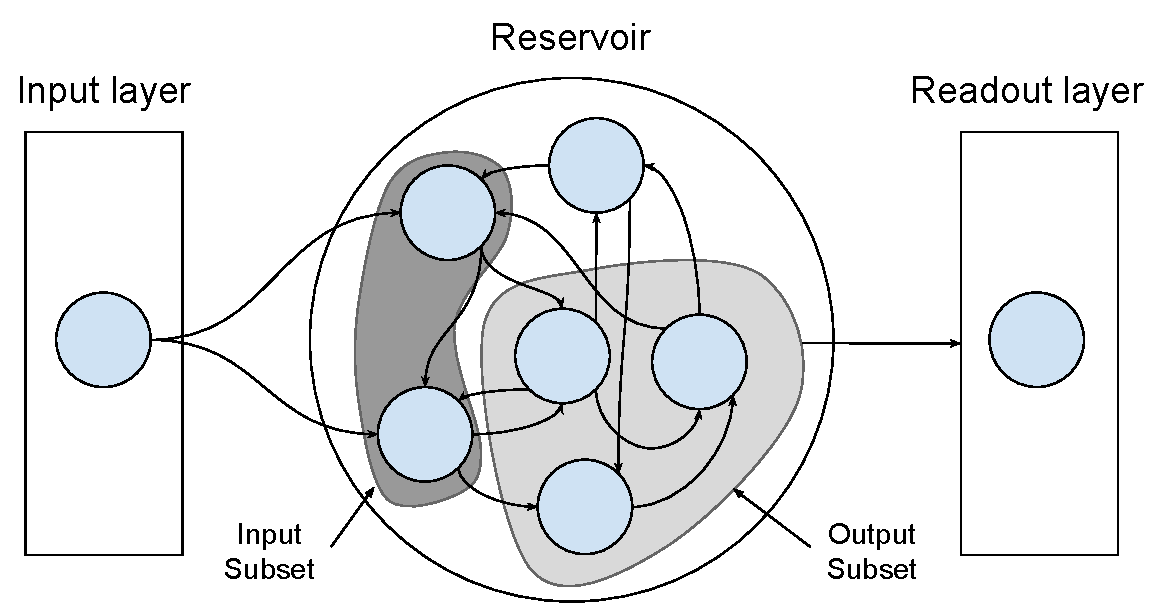
\includegraphics[width=\columnwidth]{method/rbn_reservoir_subsets.pdf}
\end{figure}

\subsection{RBN parameters and Sample sizes}

As the number of different RBNs per N-K combination is oppressively large
$(\frac{2^{2^{K}}N!}{(N-K)!})^N$ \cite{gershenson2004introduction},
the reservoir size, input, and output connectivity experiments will sample 50 RBNs for each experiment parameter combination.
This sample size was regarded adequate as a sample size of 30 was shown to give satisfactory results in \cite{burkow2015evolving}.

For the attractor analysis, the number of samples is increased to 500 per experiment parameter combination.
This larger value is chosen as the other experiments have at least 10 parameter combinations,
resulting in at least 500 samples.

Note that all our RBNs are of homogeneous connectivity,
opposed to the heterogeneous connectivity used in \cite{rbn-reservoir}.
This changes the optimal RBN connectivity for Reservoir Computing from $ \langle K \rangle = 2 $ to $ K = 3$,
as found in my pre-thesis project in section \ref{section:pre-thesis-project}.

The RBN parameters shared for all experiments are shown in table
\ref{table:shared-rbn-parameters}.

\begin{table}[h]
    \centering
    \caption{Common RBN parameters}
    \label{table:shared-rbn-parameters}
    \begin{tabular}{ll}
        \hline
        \textbf{Parameter} & \textbf{Configuration} \\
        \hline
        \hline
        Connectivity $K$ & 3   \\
        Bias $p$         & 0.5 \\
        Operation mode & CRBN (Classical synchronous RBN) \\
        \hline
    \end{tabular}
\end{table}

\subsection{Testing}

To verify that RBN simulation is working,
a RBN is created randomly, initial state set to all zeros, and ran.
The results are visualized in Figure \ref{figure:rbn-noperturb}.
We see that the RBN exhibits stable dynamics, and enters into an attractor around $t=15$.
In Figure \ref{figure:rbn-perturb} we continuously perturb the RBN with the input stream from the Temporal Parity task visualized in Figure \ref{figure:temporal-parity}.
In the perturbed case, the state trajectory is continuously changed, preventing the RBN from settling into an attractor.
Interestingly enough, there seems to be a visual similarity between the two cases.
Such a pattern is sure to disappear with a RBN in the chaotic phase.

This erratic pattern of state transitions is then fed into the readout layer,
which is then tasked with finding a linear combination of the RBN states that results in the expected output for the given task.

\begin{figure}
  \subfloat[Unperturbed]{
    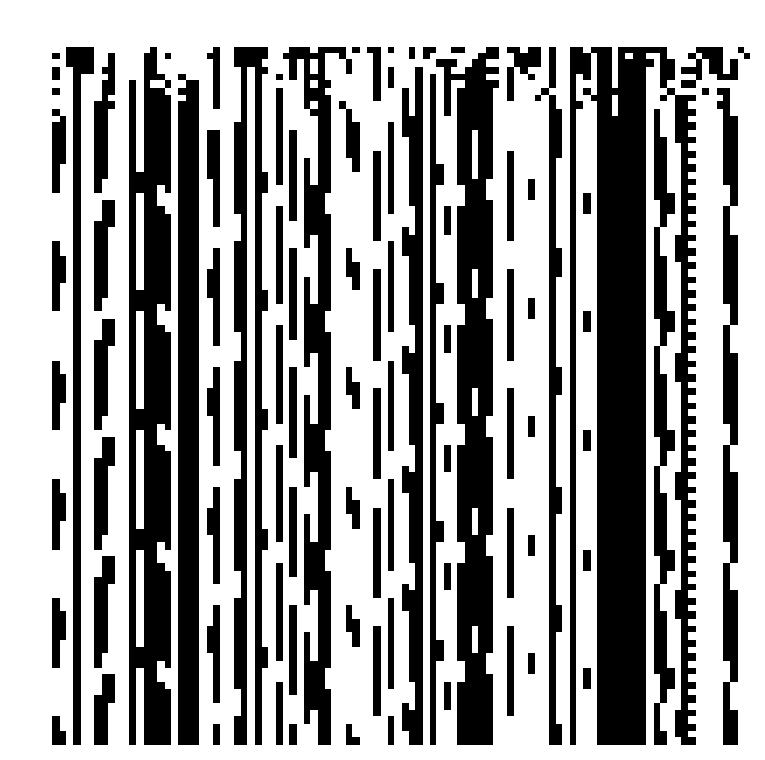
\includegraphics[width=0.5\columnwidth]{method/final-1-noperturb.pdf}
    \label{figure:rbn-noperturb}
  }
  \subfloat[Perturbed]{
    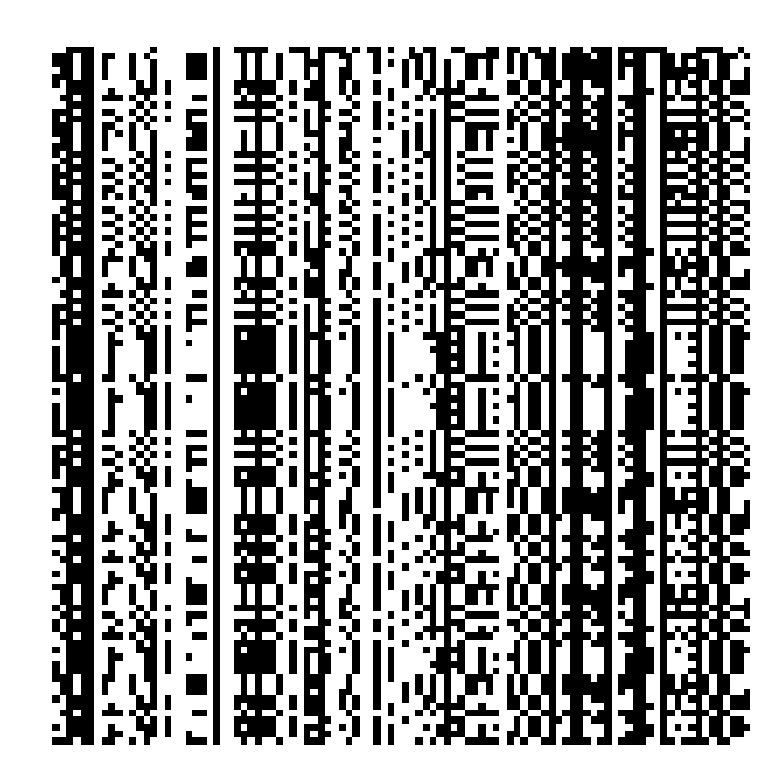
\includegraphics[width=0.5\columnwidth]{method/final-1-perturb.pdf}
    \label{figure:rbn-perturb}
  }
  \caption[Trajectories through state space for perturbed and unperturbed RBNs]{
    The same RBN ($N=100, K=2, P=0.5, IC=50$) shown both perturbed and unperturbed.
    The Boolean states of the RBN are plotted along the X-axis,
    with time flowing downwards.
  }
\end{figure}

\subsection{Training}

To train the RBN RC system we require large training datasets,
as well as different, smaller datasets for testing the trained system.
We will use the datasets described in section \ref{subsection:rbn-reservoir-systems}.

We then either create a new RBN (initialize it randomly),
or load a previously created RBN from disk.
For each bit of input in each dataset,
we perturb the input-connected nodes in the RBN.
After each perturbation, the RBN is ran synchronously (CRBN mode) for one time step.
The resulting RBN states are collected,
and after the entire dataset is processed,
forwarded to the readout layer.

To find a suitable mapping from the set of reservoir states and the correct input classification,
ridge regression \cite{hoerl1970ridge} is used.
This version of least squares regression is more accurate when faced with input collinearity, as well as always being at least as accurate as ordinary least squares.  
This process is repeated for all the datasets,
and the final regression parameters are chosen as a combination of the parameters obtained for each individual dataset.
Finally we measure the normalized accuracy of the trained reservoir on the test dataset,
defined as the following:
\begin{equation}
Accuracy = 1 - \dfrac{sum(actual\_output \neq expected\_output)}{len(correct\_output)}
\label{formula:accuracy}
\end{equation}

\subsection{Computing the attractors of an RBN}
\label{section:computing-attractors}

The number and length of attractors can vary greatly across different RBNs,
but is largely determined by the connectivity of the system \cite{gershenson2004introduction}.
There are a number of ways to estimate the number of attractors and their properties of a specific RBN.
They generally fall somewhere on the spectrum between exact enumeration (exhaustively searching for attractors from all initial states) and numerical sampling (searching from a subset only).
Numerical sampling is biased for $K\neq2$ \cite{berdahl2009random}, and cannot be used for our $K=3$ RBNs.
A brute-force exhaustive search quickly becomes infeasible, as the number of RBN states is exponential in the number of nodes.

The authors home-cooked exhaustive searcher times out for RBNs with more than 15 nodes.
A SAT-Based algorithm for finding attractors in CRBNs,
which was introduced in \cite{dubrova2011sat},
is therefore used.
It allows for an increase from 15 to 26 nodes,
which should aid in finding more meaningful results.
Its source code is available online at \cite{dubrova2011sat-online}.
